\documentclass[a4paper,11pt,spanish,leqno]{article}
\usepackage{amssymb}
\usepackage[utf8]{inputenc}
\usepackage{hyperref}
\usepackage{amsmath}
\usepackage{amssymb}
\usepackage{graphicx}
\usepackage{listings}
\title{Tarea 9}
\author{Juan Velasco Izquierdo}


\begin{document}
\maketitle
\paragraph{}\textbf{1. Sea el método Runge-Kutta: \\
$\left\{
\begin{array}{rcl}
     \xi = y_n + \frac{h}{12}(5f(t_n +\frac{h}{3},\xi) - f(t_n+h,y_{n+1})
  \\  y_{n+1} = y_n + \frac{h}{4}(f(t_n+h,y_{n+1}) + 3f(t_n+\frac{h}{3},\xi))
\end{array}
\right.$ \\
calcular la función de estabilidad y probar si el método es o no A-estable}

\paragraph{}Para calcular la función de estabilidad necesitamos obtener primero el tablero de Butcher. Ya lo tenemos calculado para este método y ese tablero es:

\[c = 
\begin{pmatrix}
	\frac{1}{3} \\
	1
\end{pmatrix} \ 
b^t = 
\begin{pmatrix}
	\frac{3}{4} & \frac{1}{4}
\end{pmatrix} \
A = 
\begin{pmatrix}
	\frac{5}{12} & -\frac{1}{12} \\
	\frac{3}{4} & \frac{1}{4}
\end{pmatrix} 
\]

Ahora simplemente tenemos que usar la fórmula de la función de estabilidad para los métodos Runge-Kutta, que es la siguiente:

\[ R(z) = (1 + zb^t(I-zA^{-1})u) = 
(1 + z
\begin{pmatrix}
	\frac{3}{4} & \frac{1}{4}
\end{pmatrix}
\left(
\begin{pmatrix}
	1 & 0 \\
	0 & 1
\end{pmatrix} 
-z
\begin{pmatrix}
	\frac{5}{12} & -\frac{1}{12} \\
	\frac{3}{4} & \frac{1}{4}
\end{pmatrix}
\right)^{-1}
\begin{pmatrix}
	1 \\
	1
\end{pmatrix} 
)=\]
\[
=(1 + z
\begin{pmatrix}
	\frac{3}{4} & \frac{1}{4}
\end{pmatrix}
\begin{pmatrix}
	\frac{-3z+12}{2z^2 -8z + 12} & -\frac{-z}{2z^2 -8z + 12} \\
	\frac{9z}{2z^2 -8z + 12} & \frac{-5z + 12}{2z^2 -8z + 12}
\end{pmatrix}
\begin{pmatrix}
	1 \\
	1
\end{pmatrix} 
)= (1 + z\frac{-z+6}{z^2-4z+61}) = \]
\[  = \frac{2z+6}{z^2-4z+6}\]

\paragraph{}Una vez tenemos la función de estabilidad vamos a aplicar el siguiente lema visto en clase para comprobar si es A-estable:
\paragraph{Lema} Sea una función racional no constante $R(z) = \frac{p(z)}{q(z)}$ ,$p$ y $q$ polinomios. Entonces $|R(z)| < 1 \ \forall z \in \mathbb{C}$ si y solo si:
\begin{enumerate}
	\item $\forall \alpha \in \mathbb{C}$ tal que $q(\alpha) = 0$ entonces $Re(\alpha) > 0$
	\item $|R(it)| \leq 1 \ \forall t \in \mathbb{R}$
\end{enumerate}

Por tanto solo tenemos que ver si las dos condiciones se cumplen o no. Para la primera vamos a coger el polinomio $q(z) = z^2-4z+6$ y vamos a hallar sus raíces como siempre: 

\[ \alpha = \frac{4 \pm \sqrt{16 - 24}}{2} = \frac{4 \pm 2\sqrt{2}i}{2}\ = 2 \pm \sqrt{2}i\]
Podemos ver que $Re(\alpha) = 2 > 0$ y por tanto $1$ se cumple.

Para la segunda condición simplemente sustituimos por $it$ y hacemos las transformaciones correspondientes para demostrarlo.

\[ \left| \frac{2ti + 6}{-t^2 - 4ti + 6} \right| \leq 1  \iff |2ti + 6|  \leq |-t^2 - 4ti + 6| \]
Calculamos el módulo para cada parte.
\[ \sqrt{6^2 + (2t)^2} \leq \sqrt{(-t^2 + 6)^2 + (4t)^2}\]
Elevamos al cuadrado cada raíz, ya que se mantendría la desigualdad.
\[ 36 + 4t^2 \leq t^4 - 12t^2 + 36 + 16t = 36 + 4t^2 + t^4 \]
Eliminamos lo que se repite a cada lado de la inecuación.
\[ 0 \leq t^4\]
Es evidente que esta desigualdad siempre se cumple $\forall t \in \mathbb{R}$ y por tanto nuestro método \textbf{es A-estable}.

\paragraph{}\textbf{2. Entregar una gráfica que muestre al menos una parte de la frontera de la región de estabilidad que justifique lo probado}

Vamos a usar Matlab para este segundo apartado. Para ello vamos a construir un mallado de números complejos entre $-10$ y $10$ para cada $x + iy$ y vamos a comprobar cuando se cumple que $|R(z)| < 1$, es decir, ver cuál es la región de estabilidad $D$ pero con esta función:
\[|2z + 6|  \leq |z^2 - 4z + 6| \]
Para los valores que lo cumpla lo guardaremos en unos nuevos vectores y finalmente los representaremos como puntos. El código es el siguiente:
\begin{lstlisting}[language=Matlab]
x = linspace(-10,10,1000);
y = linspace(-10,10,1000);
x_new = [];
y_new = [];
for i = 1 :size(x,2)
    for j = 1 :size(y,2)
        if abs((2*complex(x(i),y(j)) + 6))< 
            abs(((complex(x(i),y(j)))^2 -4*complex(x(i),y(j)) + 6)) 
            x_new(end+1) = x(i);
            y_new(end+1) = y(j);
        end
    end
end
plot(x_new,y_new,'o')
\end{lstlisting}

La imagen que ha resultado es la siguiente:

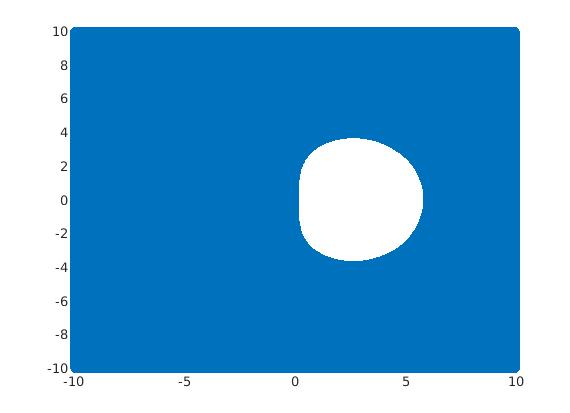
\includegraphics[scale=0.5]{Tarea9.jpg}

Como podemos ver la región de estabilidad $D$, que viene dada por el color azul, es todo el
cuadrado $[-10,10]$ salvo la forma blanca del centro. Vemos también que $ \mathbb{C}_-
\subset D$ y por tanto es \textbf{A-estable} (como habíamos determinado antes) y la frontera de $D$, $\partial D$, \textbf{es el contorno de la figura blanca}.
\end{document}
